\chapter{Diseño electrónico del sistema}
\ihead[]{Capítulo 4: Diseño electrónico del sistema}
\label{ch:CH04-Diseno-Electronico}
%%%%%%%%%%%%%%%%%%%%%%%%%%%%%%%%%%%%%%%%%%
En este capítulo se desarrollará el diseño electrónico de los subsistemas del concepto de solución óptima, incluyendo la selección de los componentes necesarios para el funcionamiento del sistema. Asimismo, se establecen las consideraciones de diseño de una \ac{PCB} a medida que integre los componentes definidos, tomando como base las pruebas en prototipo y la documentación técnica de cada componente elegido.
\section{Selección de componentes electrónicos}
    El \ac{HW} del sistema realizará tres tareas principales: energizar el motor de pruebas, sensar sus variables físicas (voltaje, corriente y velocidad angular) y enviar los datos del sensado de variables hacia la interfaz. Por ello, se comenzará realizando la selección de componentes que permitan realizar las tareas.
    \subsection{Selección de microcontrolador}
        Para iniciar el diseño se definirá el microcontrolador a utilizar. Como se presentó en la matriz morfológica \ref{fig:Annex_E_MatrizMorfologica-05-control} del Anexo \ref{an:Anexo_G_MatrizMorfologica}, se consideraron dos opciones: un microcontrolador y una \ac{SBC}. Por criterios de costo expuestos en la sección \ref{sec:solucion_optima}, y dado que durante la experiencia de registro de datos se desarrollará una interfaz de escritorio para controlar el \ac{HW} desde la \ac{PC} del usuario, se descartó la opción de utilizar una \ac{SBC}. En consecuencia, se evalúan tres opciones de microcontroladores comerciales: placas de desarrollo basadas en la familia ATmega (Arduino), el microcontrolador ESP32 y la placa de desarrollo STM32F103C8T6 de la familia de microcontroladores STM32. A continuación, en la Tabla \ref{tab:mcus} se presentan estas tres alternativas para el desarrollo de la PCB de control del \ac{HW} y sus principales características.
        
        \begin{longtblr}[theme=pucp,
          label   = {tab:mcus},
          caption = {Comparativa de microcontroladores para el banco de pruebas (IO, adquisición y conectividad)},
        ]{
          colspec = {X[c,m] X[l,m] X[l,m] X[l,m]}, % 1ª centrada, resto a la izq.
          colsep=3pt,
          row{1}={halign=c},
          rowhead=1, rowfoot=0,
          hlines, vlines,
        }
        Característica
          & 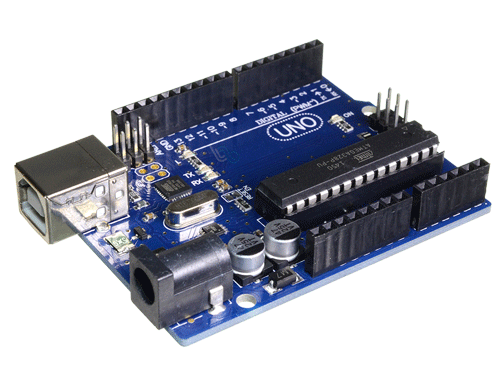
\includegraphics[width=2.5cm]{CHPTRS/CH04_DIS_ELECTRONICO/Componentes/ArduinoUNO.png} Arduino UNO R3 (Atmega328P)
          & \includegraphics[width=2.5cm]{CHPTRS/CH04_DIS_ELECTRONICO/Componentes/DIS_ELEC_01_ChipESP32-32D.jpg} ESP32-WROOM-32D
          & 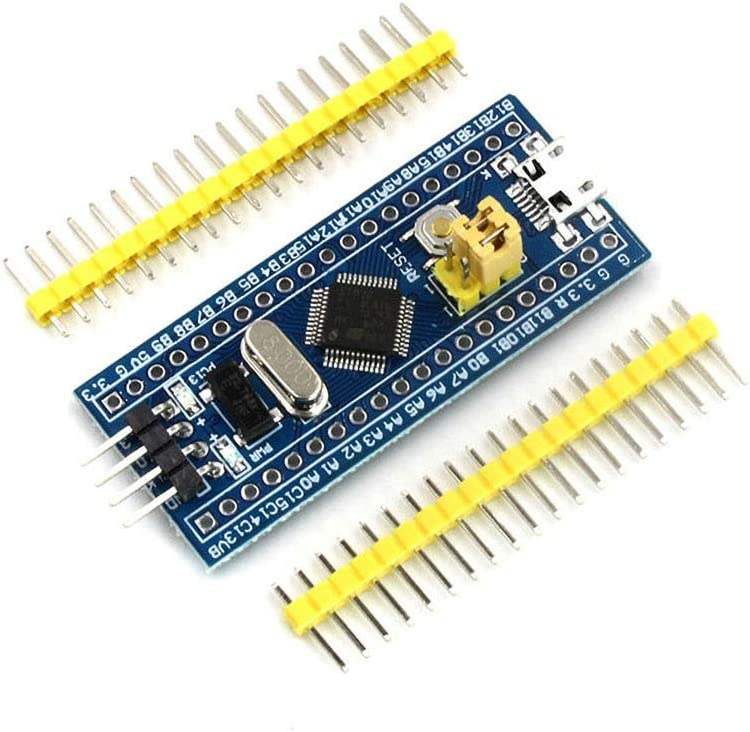
\includegraphics[width=2.5cm]{CHPTRS/CH04_DIS_ELECTRONICO/Componentes/STM32.jpg} STM32F103C8T6\\
        Arquitectura / núcleos
          & AVR 8 bit, 1 núcleo hasta 16\,MHz
          & Xtensa LX6, 2 núcleos hasta 240\,MHz
          & Arm Cortex-M3 32 bit hasta 72\,MHz \\
        Memoria
          & Flash 32\,KB, SRAM 2\,KB, EEPROM 1\,KB
          & SRAM 520\,KB, 4\,MB SPI flash en el módulo
          & Flash 64\,KB (algunas placas 128\,KB); SRAM 20\,KB \\
        ADC / DAC
          & ADC 10 bit (6 canales), sin DAC
          & 2 SAR ADC 12 bit (hasta 18); 2 DAC 8 bit
          & 2 ADC 12 bits (hasta 16 canales); sin DAC \\
        Comunicaciones
          & UART, SPI, $I^2C$
          & SPI, $I^2C$, UART, SDIO, TWAI (CAN 2.0), MAC Ethernet\footnotemark[1]
          & SPI, $I^2C$, USART/UART, CAN 2.0B, USB FS \\
        Temporizadores / PWM
          & 6 salidas PWM
          & LEDC PWM, MCPWM
          & hasta 7 temporizadores (PWM/IC/OC, interfaz de encoder; TIM1 avanzado) \\
        Conectividad RF
          & No cuenta con esta funcionalidad & Wi-Fi 802.11 b/g/n + Bluetooth v4.2 BR/EDR + BLE & No cuenta con esta funcionalidad \\
        Voltaje de operación (IO)
          & 5\,V (IO 5\,V)
          & 3.0 – 3.6\,V (IO 3.3\,V)
          & 2.0 – 3.6\,V (IO 3.3\,V; \emph{algunos pines toleran 5\,V}) \\
        Entorno de desarrollo
          & Arduino IDE
          & ESP-IDF (oficial) / Arduino Core
          & STM32CubeIDE/HAL (opcional Arduino Core STM32) \\
        Precio (moneda local S/)
          & S/ 25 & S/ 30 & S/ 25 \\
        \end{longtblr}
        \footnotetext[1]{Microcontrolador ESP32 incorpora interfaz MAC Ethernet (RMII); sin embargo requiere un PHY externo.}
        % \begin{figure}[H]
        %     \centering
        %     \begin{tabularx}{\linewidth}{>{\centering\arraybackslash}X}
        %         % Fila 1: imagen
        %         \begin{subfigure}[t]{\linewidth}
        %             \centering
        %             \includegraphics[width=0.35\linewidth]{CHPTRS/CH04_DIS_ELECTRONICO/Fig_Componentes/DIS_ELEC_01_ChipESP32-32D.jpg}
        %         \end{subfigure}
        %     \end{tabularx}
        %     \caption{Microcontrolador ESP32-WROOM-32}
        %     \label{fig:black_box}
        % \end{figure}
        Se utilizará el microcontrolador ESP32-32D montado en una placa propia y programable mediante USB-C gracias a un convertidor USB–TTL CH340 configurado a 3.3\,V. El \textit{chip} CH340 ofrece interfaz USB que se enumera como puerto serie virtual y habilita carga de firmware. El diseño de este  Además, el microcontrolador ESP32 aporta doble núcleo (hasta 240\,MHz), SRAM integrada, ADC de 12 bits, temporizadores y periféricos PWM para el control del puente H, además de SPI para los periféricos de adquisición (sensor magnético y módulo Ethernet). En cuanto al \ac{SW}, la plataforma admite FreeRTOS y capacidades de tiempo real, disponibles pero no necesariamente empleadas en este proyecto. La combinación USB-C con CH340 para programación y comunicación serie, junto con las interfaces SPI, PWM y ADC del ESP32, satisface los requisitos del banco de pruebas para el sensado y la transmisión de datos hacia la \ac{PC}.
        \begin{figure}[H]
            \centering
            \begin{tabularx}{\linewidth}{>{\centering\arraybackslash}X}
                % Fila 1: imagen
                \begin{subfigure}[t]{\linewidth}
                    \centering
                    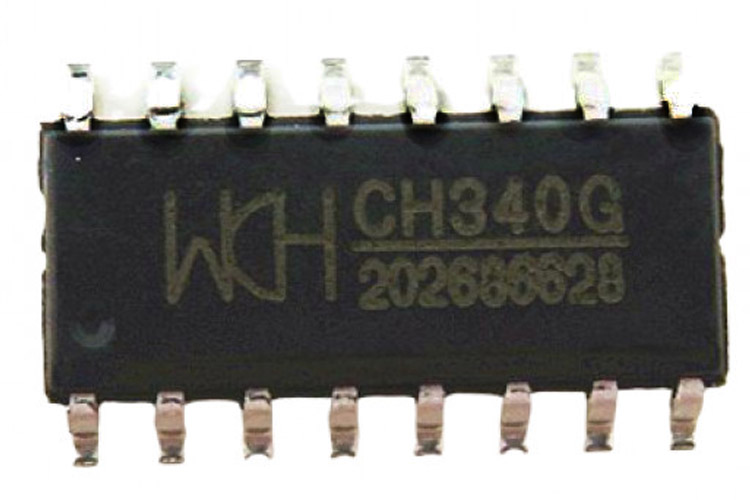
\includegraphics[width=0.4\linewidth]{CHPTRS/CH04_DIS_ELECTRONICO/Fig_Componentes/DIS_ELEC_02a_ChipCH340.jpg}
                \end{subfigure}
            \end{tabularx}
            \caption{Integrado CH340 cargar el programa y de poder comunicarse con el micrcontrolador elegido}
            \label{fig:black_box}
        \end{figure}
    \subsection{Selección de sensor de efecto \textit{hall}}
        Como se mencionó en la sección \ref{sec:solucion_optima} del Capítulo \ref{ch:CH03-Diseno-Conceptual} se utilizarán sensores de efecto \textit{hall} para medir la velocidad angular del motor. Este sensor a elegir debe ser lo suficientemente rápido para medir los cambios en la velocidad del motor, ya que como se puede observar en el Capítulo \ref{ch:CH07_Implementacion}, los motores \ac{DC} son sistemas que reaccionan muy rápido y estabilizan sus variables en poco tiempo (aquí se referenciaran secciones del Capítulo \ref{ch:CH07_Implementacion} que contengan gráficas de velocidad de los motores a probar)
        se seleccionó el TMAG5170 por cuatro razones alineadas al diseño del prototipo:
        \begin{itemize}
        \item Alta razón de muestreo y baja latencia. Su conversión rápida (orden de decenas de \si{\micro\second}) y lectura permiten explotar la capacidad de servicio de interrupciones de la ESP32, de modo que el lazo de adquisición (Cap. \ref{ch:CH07_Implementacion}) estima velocidad angular con retraso despreciable respecto a la dinámica del motor. 
        \item Versatilidad funcional. Aunque el diseño original contemplaba un disco con imanes para detectar flancos (disco con imanes en el eje del motor), la disponibilidad del ángulo (\(0\text{–}360^\circ\)) y la habilitación selectiva de ejes X–Y–Z permiten simplificar el \ac{HW}: se reemplaza el conteo de flancos por medición angular directa del imán montado en el eje. 
        \item Compatibilidad eléctrica y de integración. Su alimentación entre \SI{2.3}{\volt} y \SI{5.5}{\volt} y niveles lógicos referidos a V\textsubscript{CC} facilitan operar con el microcontrolador seleccionado a \SI{3.3}{\volt}. Además, que simplifica el hecho de utilizar una etapa extra de regulación aparte de la que energiza al microcontrolador y los demás módulos. 
        \item Interfaz \ac{SPI} . La comunicación serie síncrona se puede implementar con el microcontrolador seleccionado tanto para la programación del sensor como para recibir los datos de velocidad angular
        \end{itemize}
        \ref{sec:solucion_optima}.
        \begin{figure}[H]
            \centering
            \begin{tabularx}{\linewidth}{>{\centering\arraybackslash}X}
                % Fila 1: imagen
                \begin{subfigure}[t]{\linewidth}
                    \centering
                    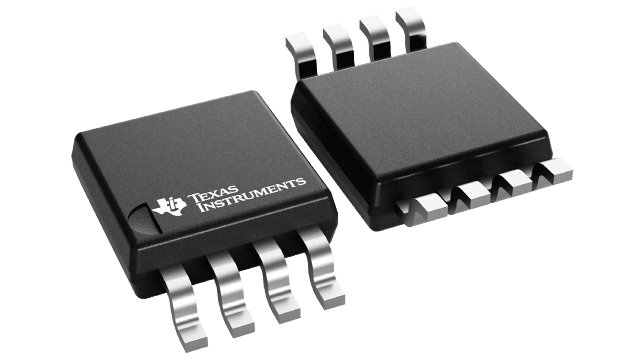
\includegraphics[width=0.4\linewidth]{CHPTRS/CH04_DIS_ELECTRONICO/Fig_Componentes/DIS_ELEC_03a_ChipTMAG.jpg}
                \end{subfigure}
            \end{tabularx}
            \caption{Imagen del sensor de efecto \textit{hall} TMAG5170}
            \label{fig:black_box}
        \end{figure}
    \subsection{Selección de \textit{driver} de motor}
        De mismo modo que con el microcontrolador y el sensor a utilizar, se procederá a elegir un \textit{driver} para el control de los motores a caracterizar, en este caso se opta por 3 alternativas, 2 \textit{chips} que los venden como módulos de desarrollo en el mercado local y otro que es un integrado de puente H de alta \textit{performance} para motores utilizados en la industria y el sector automotriz:
        \begin{longtblr}[theme=pucp,
          label   = {tab:hbridge_comp},
          caption = {Comparativa de drivers de potencia para motor \ac{DC}},
        ]{
          colspec = {X[c,m] X[l,m] X[l,m] X[l,m]}, % 1ª centrada, resto a la izq.
          colsep=3pt,
          row{1}={halign=c},
          rowhead=1, rowfoot=0,
          hlines, vlines,
        }
            Característica
          & 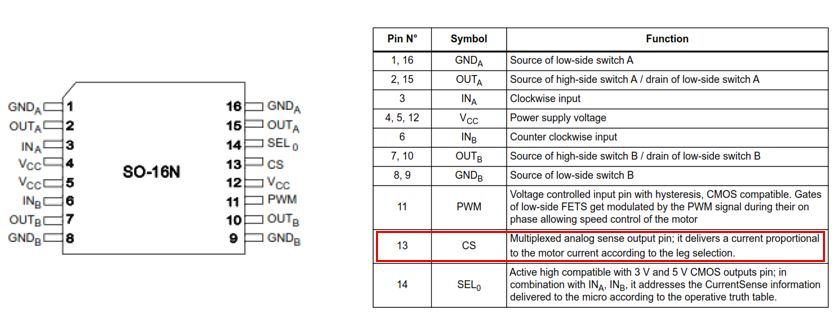
\includegraphics[width=2.5cm]{CHPTRS/CH04_DIS_ELECTRONICO/Fig_Componentes/DIS_ELEC_06_DriverVNH.jpg} VNH7070BAS
          & 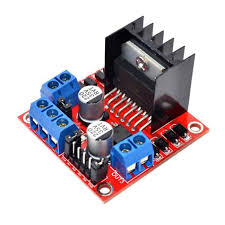
\includegraphics[width=2.5cm]{CHPTRS/CH04_DIS_ELECTRONICO/Componentes/L298N.jpeg} L298N
          & 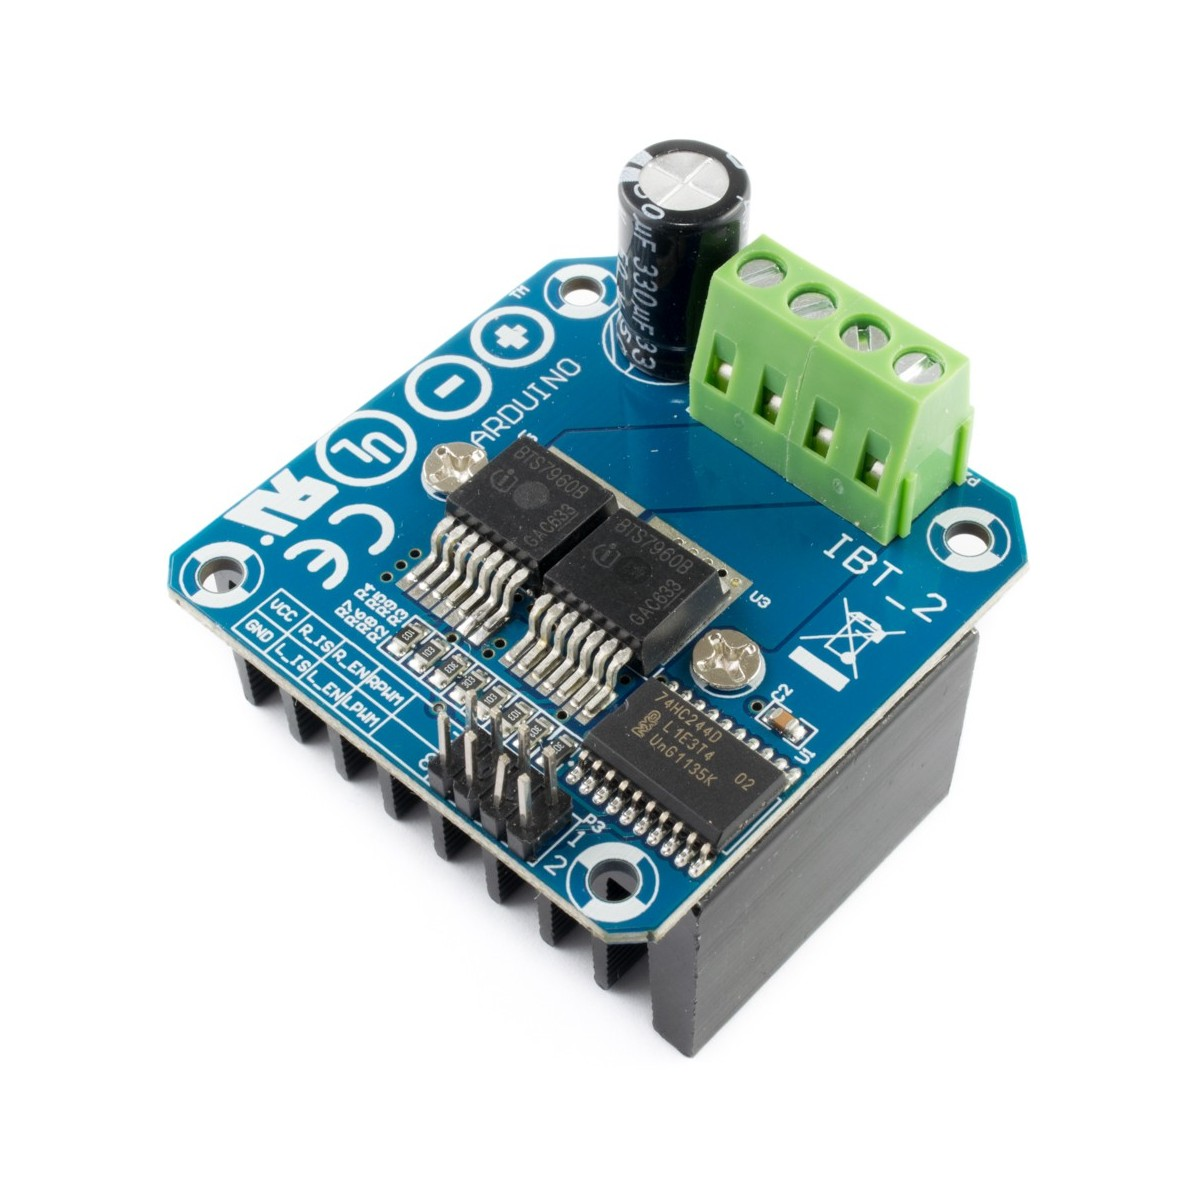
\includegraphics[width=2.5cm]{CHPTRS/CH04_DIS_ELECTRONICO/Fig_Componentes/DIS_ELEC_04B_DriverBTS7960.jpg} BTS7960\\
            Topología
              & Puente H completo integrado (4 MOSFET de potencia)
              & Doble puente H con transistores bipolares (BJT)
              & Medio puente (se requieren \emph{dos} para formar un puente H) \\
            Tecnología de potencia
              & MOSFET automotriz (VIPower M0-7)
              & Transistores BJT de potencia
              & MOSFET (NovalithIC: P-canal alta, N-canal baja) \\
            Alimentación típica
              & \(V_{\mathrm{CC}}\) de 4--28\,V
              & Hasta 46\,V (lógica a 5\,V)
              & Operativo 5.5--27.5\,V \\
            Entradas lógicas
              & Umbrales CMOS (\(V_{\mathrm{IH}}\sim 2.1\,\mathrm{V}\), \(V_{\mathrm{IL}}\sim 0.9\,\mathrm{V}\)); compatible 3.3\,V
              & TTL; lógica a 5\,V (\(V_{\mathrm{IH}}\ge 2.3\,\mathrm{V}\))
              & TTL/CMOS; pines IN/INH \\
            PWM
              & Entrada PWM  (frecuencia máxima de 20 kHz)
              & Soporta conmutación, pero con pérdidas elevadas por BJT
              & PWM hasta (frecuencia máxima de 25  kHz) \\
            Sensado de corriente
              & Sí, pin CS brinda una corriente proporcional a la del motor
              & Pines “Sense” para resistores externos; \emph{no} hay espejo/ganancia integrada
              & Sí, pin IS brinda corriente proporcional a la del motor  \\
            Protecciones
              & Sobre-corriente, sobre-temperatura y protección sobre-corriente en caso de cortocircuito
              & Sobre-temperatura
              & \textit{Current limit} (\(\approx \SI{43}{A}\)), sobre-temperatura; \emph{dead-time} interno \\
            Integración / BOM
              & Un solo CI para un motor bidireccional $+$ sensado
              & Un solo CI, pero con diodos externos y pérdidas altas
              & Dos CI para un puente H completo (uno por rama) \\
       \end{longtblr}
       \begin{figure}[H]
            \centering
            \begin{tabularx}{\linewidth}{>{\centering\arraybackslash}X}
                % Fila 1: imagen
                \begin{subfigure}[t]{\linewidth}
                    \centering
                    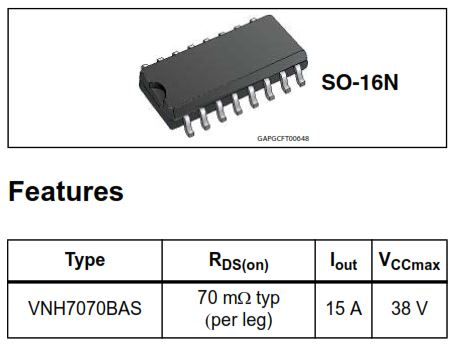
\includegraphics[width=0.5\linewidth]{CHPTRS/CH04_DIS_ELECTRONICO/Fig_Componentes/DIS_ELEC_05_DriverVNH.jpg}
                \end{subfigure}
            \end{tabularx}
            \caption{Integrado CH340 cargar el programa y de poder comunicarse con el micrcontrolador elegido}
            \label{fig:black_box}
        \end{figure}
    \subsection{Selección de sensor de corriente}
        Se adopta el sensado de corriente integrado del puente H VNH7070BAS, el cual presenta en el pin CS una señal proporcional a la corriente del motor. Esta elección elimina la necesidad de un sensor de corriente \ac{DC} adicional y reduce complejidad y ocupación en la \ac{PCB}.         
        En la sección \ref{sec:diseño_driver} se diseña un pequeño circuito de adecuación para que la señal de CS sea compatible con el ADC del microcontrolador (\SI{0}{\volt}–\SI{3.3}{\volt})
        \begin{figure}[H]
            \centering
            \begin{tabularx}{\linewidth}{>{\centering\arraybackslash}X}
                % Fila 1: imagen
                \begin{subfigure}[t]{\linewidth}
                    \centering
                    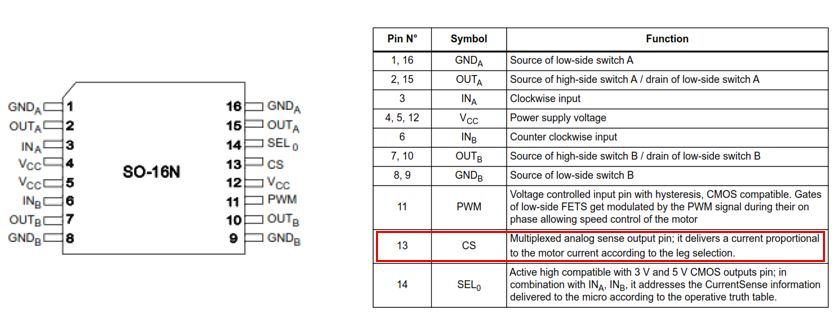
\includegraphics[width=0.75\linewidth]{CHPTRS/CH04_DIS_ELECTRONICO/Fig_Componentes/DIS_ELEC_06_DriverVNH.jpg}
                \end{subfigure}
            \end{tabularx}
            \caption{Integrado CH340 cargar el programa y de poder comunicarse con el micrcontrolador elegido}
            \label{fig:black_box}
        \end{figure}
        Finalmente, en el capítulo de implementación se calibrará la ganancia real del sensado (\(K_{\text{CS}}\)) y su posible offset mediante ensayos comparativos con un sensor de corriente de referencia. Con dichos datos se ajustará el modelo de conversión a la forma
        \[
        I_{\text{motor}} = \alpha\,V_{\text{ADC}} + \beta,
        \]
        dejando documentados \(\alpha\) (ganancia efectiva) y \(\beta\) (offset) para mejorar la exactitud de las mediciones en las pruebas del prototipo.

    \subsection{Selección de fuente de alimentación}

        Dado el requisito de conexión directa a red (\SI{220}{\volt}–\SI{60}{\hertz}), se seleccionó una \ac{SMPS} en lugar de una fuente lineal. Las \ac{SMPS} ofrecen mayor eficiencia y densidad de potencia, reduciendo volumen y masa al prescindir del transformador de \SI{60}{\hertz} propio de las topologías lineales; estas características favorecen la integración del sistema en un chasis compacto (véase \cite{fswitchignfuentelineal}). 
        \begin{figure}[H]
            \centering
            \begin{tabularx}{\linewidth}{>{\centering\arraybackslash}X}
                % Fila 1: imagen
                \begin{subfigure}[t]{\linewidth}
                    \centering
                    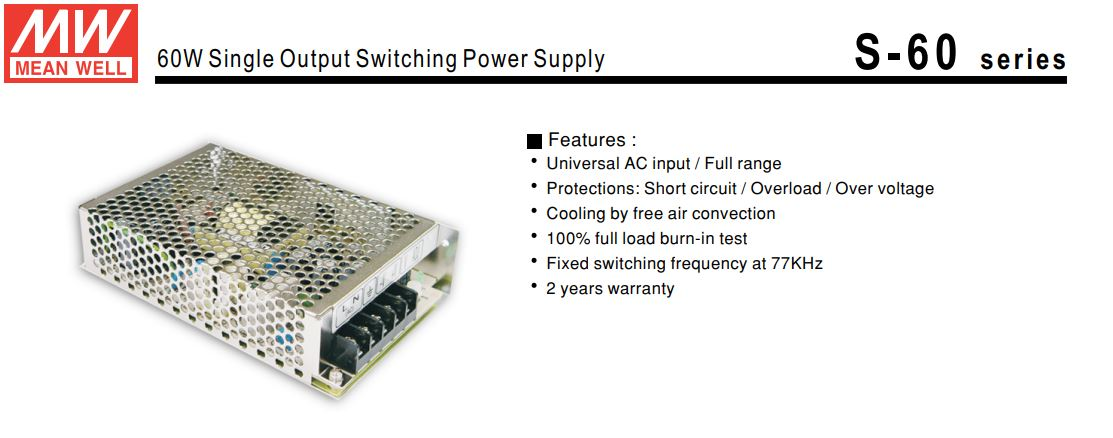
\includegraphics[width=0.5\linewidth]{CHPTRS/CH04_DIS_ELECTRONICO/Fig_Componentes/DIS_ELEC_07_FuenteSwitching.jpg}
                \end{subfigure}
            \end{tabularx}
            \caption{Fuente \textit{switching} elegida para alimentar la \ac{PCB} de control}
            \label{fig:smps}
        \end{figure}
        En particular, se empleará la MEAN WELL serie S-60 mopstrada en la Figura \ref{fig:smps}, con entrada universal \SI{85}{\volt}–\SI{264}{\volt}~\ac{AC} y protecciones contra cortocircuito, sobrecarga y sobretensión, por lo que no es necesario diseñar desde cero la etapa \ac{AC}/\ac{DC}. El modelo específico es el S-60-12 se selecciona según la tensión y potencia requeridas por los módulos del sistema, manteniendo margen de diseño.
\section{Diseño de \ac{PCB}}
    En esta sección se diseñan los circuitos necesarios para la implementación del banco de pruebas, los cuales se estructuran en coherencia con los dominios definidos en el Capítulo \ref{ch:CH03-Diseno-Conceptual}. En particular, se aborda: (i) la etapa de regulación de voltaje para la alimentación distribuida de los módulos, (ii) la electrónica de control empleada durante la caracterización del motor, (iii) la interfaz de comunicación con el \ac{SW}, y (iv) el acondicionamiento y la adquisición de señales de los sensores necesarios para la extracción de datos del motor.
    \subsection{Diseño de circuitos de potencia}
        Para energizar todo el sistema de control se requiere regular el voltaje que entrega la fuente \textit{switching}, la cual proporciona \SI{12}{\volt} \ac{DC}. Dado que el microcontrolador ESP32, el sensor y el módulo Ethernet operan a \SI{3.3}{\volt}, se empleará una fuente \ac{DC}-\ac{DC} de topología \textit{buck}. Como se muestra en la Figura \ref{fig:RegDeVoltaje}, se utiliza el regulador LM2594 junto con los componentes propios de una fuente \textit{buck}.
        \begin{figure}[H]
           \centering
           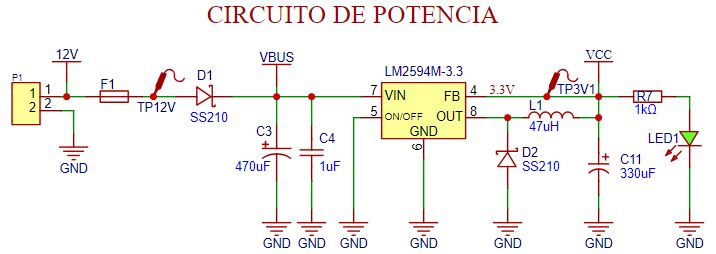
\includegraphics[width=1\textwidth]{CHPTRS/CH04_DIS_ELECTRONICO/Fig_Esquematicos/DIS_ELEC_01_CircuitoDePotencia.jpg}
           \caption{Diagrama esquemático del regulador de voltaje de la \ac{PCB} de control}
           \label{fig:RegDeVoltaje}
        \end{figure}
        Los valores de los capacitores y bobinas que acompañan al integrado LM2594 son provistos y ya están calculados por el fabricante, como se muestra en la Figura \ref{fig:CircuitoDeRegulacion}. Además de estos componentes, en la Figura \ref{fig:RegDeVoltaje} se incluye un fusible para proteger ante sobrecorrientes toda la \ac{PCB} de control, así como un LED indicador del estado de energización del sistema.
        \begin{figure}[H]
           \centering
           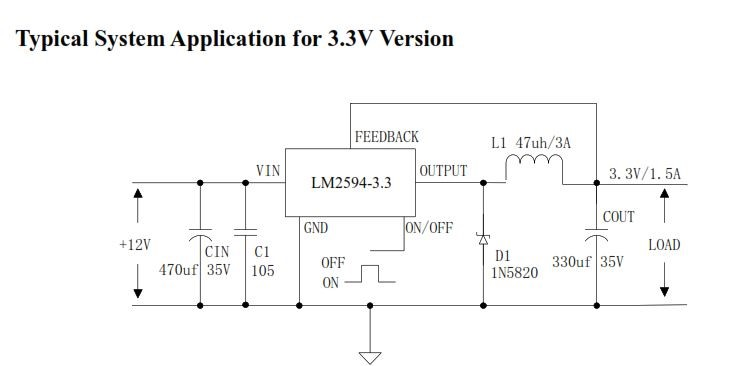
\includegraphics[width=1\textwidth]{CHPTRS/CH04_DIS_ELECTRONICO/Fig_Esquematicos/DIS_ELEC_01_CircuitoDePotenciaRecomendado.jpg}
           \caption{Diseño típico de regulador LM2594}
           \label{fig:CircuitoDeRegulacion}
        \end{figure}
    \subsection{Diseño de circuitos de control}
        Para la parte de control se utilizará el chip de la ESP32-32D, donde el primer paso es investigar sobre su distribución de pines y características de su \textit{datasheet}. Para ello, en la Figura \ref{fig:PinesESP32} se muestra la distribución de pines y las funciones que estos cumplen como se detalla a continuación:
        \begin{itemize}
          \item Pines digitales: entradas/salidas lógicas (0/1), con posibilidad de interrupciones y \textit{pull-up}/\textit{pull-down} configurables.
          \item Pines analógicos: lectura de señales continuas mediante ADC de 12 bits, convirtiéndolas en valores digitales procesables.
          \item Pines PWM: generación de señales con ciclo útil variable para controlar velocidad de motores o intensidad de LEDs.
          \item Pines de alimentación: VCC (3.3\,V) y GND, indispensables para el funcionamiento del módulo.
          \item Pines de comunicación: interfaces UART (TX/RX), SPI (MOSI/MISO/SCK/CS) e I\textsuperscript{2}C (SDA/SCL) para intercambio de datos con periféricos.
        \end{itemize}
        \begin{figure}[H]
            \centering
            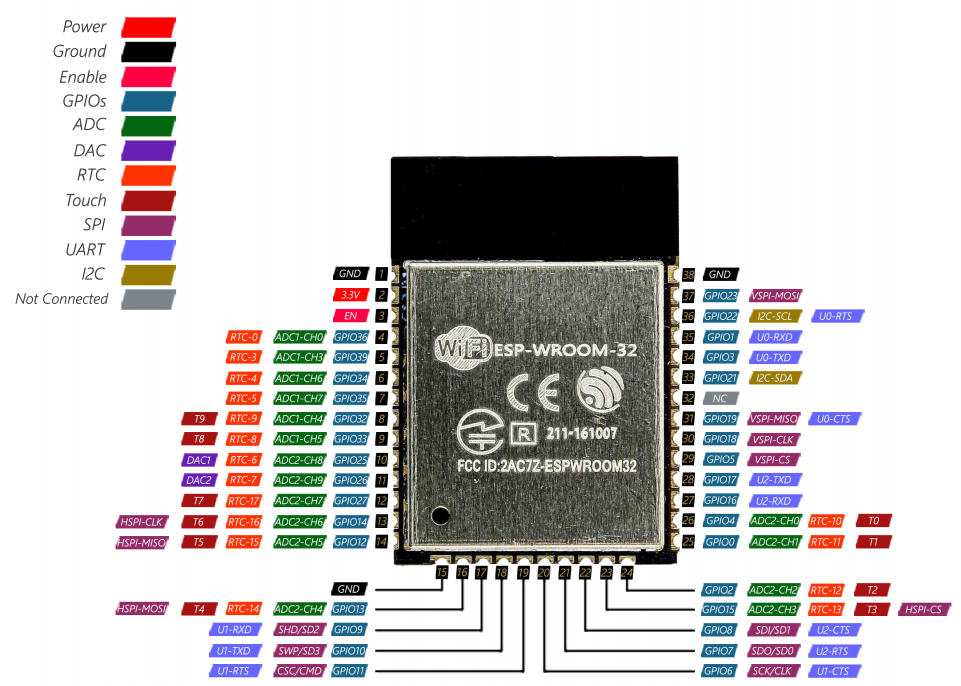
\includegraphics[width=0.7\textwidth]{CHPTRS/CH04_DIS_ELECTRONICO/Fig_Pinout/PINOUT_01_ESP32.png}
            \caption{Pinout del microcontrolador ESP32}
            \label{fig:PinesESP32}
        \end{figure}
        Para esta aplicación se empleará un único bus SPI compartido entre la ESP32, el sensor TMAG7051 y el módulo Ethernet ENC28J60 (véase el Anexo \ref{an:Anexo_J_ComunicacionSPI}). Se asignan GPIO18 como SCK, GPIO23 como MOSI y GPIO19 como MISO; y líneas de selección independientes: GPIO5 como CS del TMAG7051 y GPIO22 como CS del ENC28J60. Opcionalmente, el pin INT del ENC28J60 puede conectarse al GPIO27 para notificación de eventos. Todos los módulos operan a 3.3,V y comparten una tierra común. Estas conexiones se muestran en la Figura \ref{fig:DiagramaConexiones}, correspondiente al esquema de la \ac{PCB} de control.
        \begin{figure}[H]
            \centering
            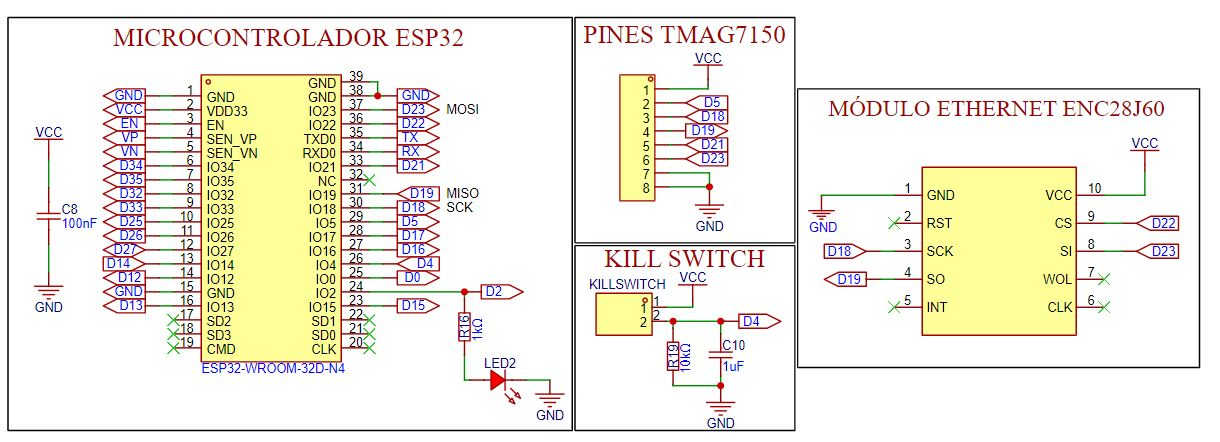
\includegraphics[width=1\textwidth]{CHPTRS/CH04_DIS_ELECTRONICO/Fig_Esquematicos/DIS_ELEC_04_CircuitoDeConexiones.jpg}
            \caption{Diagrama de conexiones entre el microcontrolador, módulo de Ethernet y sensor de efecto \textit{hall} TMAG5170}
            \label{fig:DiagramaConexiones}
        \end{figure}
    \subsection{Diseño de circuito para VNH7070BAS}
    \label{sec:diseño_driver}
        Para controlar el puente H se emplearán pines de la ESP32 para el ciclo de trabajo, la habilitación de sentidos de giro y la medición de corriente. El integrado requiere dos referencias unidas en un punto estrella: tierra de señal (microcontrolador, GPIO y \ac{PWM}) y tierra de potencia de la fuente del motor.
        \begin{figure}[H]
            \centering
            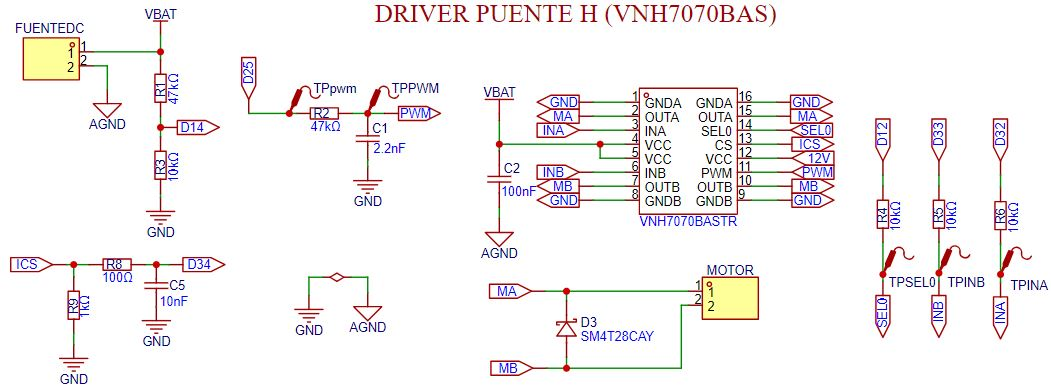
\includegraphics[width=1\textwidth]{CHPTRS/CH04_DIS_ELECTRONICO/Fig_Esquematicos/DIS_ELEC_03_CircuitoDeDriverPuenteH.jpg}
            \caption{Diagrama esquemático de conexiones con el driver VNH7070BAS}
            \label{fig:DiagramaConexiones}
        \end{figure}
        VBAT recibe el voltaje nominal del motor. Se coloca un condensador cerámico de \SI{100}{\nano\farad} lo más próximo posible a VBAT–AGND y, en la entrada, un condensador electrolítico (\SI{47}{\micro\farad}–\SI{220}{\micro\farad}) para amortiguar el transitorio. La alimentación lógica VCC (3,3–5V) lleva su propio \SI{100}{\nano\farad} junto a los pines del CI. Dado que no tolera polaridad inversa, se recomienda protección de entrada (MOSFET de protección o diodo serie) según la caída de tensión admisible.
        
        El TVS SM4T28CAY se conecta entre MA y MB el cual sirve como un diod de protección que se conecta en paralelo al motor para disipar las corrientes que almacene el motor luego de su uso, para que estas no se devuelvan al driver y que mas bien se consuman con el diodo.
        
        INA, INB, \ac{PWM} y SEL0 se conectan a GPIO de la ESP32 con resistencias \textit{pull-down} de \SI{10}{\kilo\ohm} para evitar estados flotantes al arranque. La \ac{PWM} opera típicamente entre 10–20 kHz; si es necesario mitigar EMI, se limita el \textit{slew rate} con una red RC pequeña cerca del pin . Evitar redes que promedien la \ac{PWM}, pues distorsionan el ciclo efectivo en una entrada digital.
        
        El pin CS entrega una corriente proporcional a la corriente de fase \(I_{\text{OUT}}\) con factor \(K_{\text{ILIS}}\). Se convierte a tensión con una resistencia \(R_{\text{CS}}\) a GND y se filtra con un condensador (R8 y C5 como filtro \textit{anti-aliasing}):
        \[
        V_{\text{CS}} = I_{\text{OUT}}\cdot K_{\text{ILIS}}\cdot R_{\text{CS}}.
        \]
        Al dimensionar \(R_{\text{CS}}\), garantizar \(V_{\text{CS}}\leq V_{\text{ADC,max}}\) (\SI{3.3}{\volt}) para la corriente máxima y respetar el límite del pin CS (\(\leq\) 10 mA \ac{DC}). Para precisión, el retorno de CS y el GND del ADC deben ir por conexión Kelvin al punto estrella.
        
        Los bornes del motor se conectan a MA/MB. El bucle de alta corriente (Vbat hacia el motor) debe ser lo más corto y compacto posible; en PCB, usar plano de potencia, \textit{vias} térmicas bajo el CI y anchos de pista acordes a la corriente. Durante el arranque, establecer un estado seguro: INA = INB = 0 y \ac{PWM} = 0 hasta completar la inicialización.
        
        El VNH7070BAS integra limitación de corriente, protección de cortocircuito y \textit{thermal shutdown} con \textit{auto-retry}. Son funciones de protección y no sustituyen el control de corriente de la aplicación; para un límite programable se cierra un lazo digital leyendo CS y modulando la \ac{PWM} en \textit{firmware}.

    
    \subsection{Diseño de circuitos para el sensor de efecto \textit{hall} TMAG5170}
        La placa integra el sensor TMAG5170 y lo conecta con la placa principal (ESP32) mediante un conector de ocho vías. La alimentación es de 3.3 V y se comparte la referencia de masa con la placa principal. El acondicionamiento local incluye dos condensadores de desacoplo próximos entre VCC y GND del CI: C8 = 100 nF (alta frecuencia) y C2 = 1 µF (baja impedancia a media y baja frecuencia). La interfaz SPI se enruta en cuatro hilos (SCK, SDI/MOSI, SDO/MISO y CS); para mejorar la integridad de señal se añade una resistencia en serie R4 = 100 ohm en SCK, colocada cerca del TMAG5170, que atenúa los flancos y reduce el “ringing” sin afectar el temporizado. El pin ALERT, de tipo drenador abierto, se eleva con un pull-up R5 = 4.7 kohm a 3.3 V para indicar “data-ready” o diagnóstico hacia el microcontrolador. El pin TEST se fija a GND según la recomendación del fabricante. Todas las señales operan a niveles CMOS de 3.3 V; se recomienda mantener las pistas del bus cortas, con retorno de masa directo bajo cada traza y alejadas del lazo de potencia del puente H. Mecánicamente, para la medición on-axis (imán diametral coaxial al encapsulado), la placa debe alinearse de modo que el centro del imán coincida con el centro del CI y con holgura axial estable; esta orientación permite estimar el ángulo en el plano XY con mínima elipticidad. La lectura angular puede obtenerse directamente del TMAG5170 o calcularse en la ESP32 a partir de Bx y By mediante la función atan2(By, Bx).

        \begin{figure}[H]
           \centering
           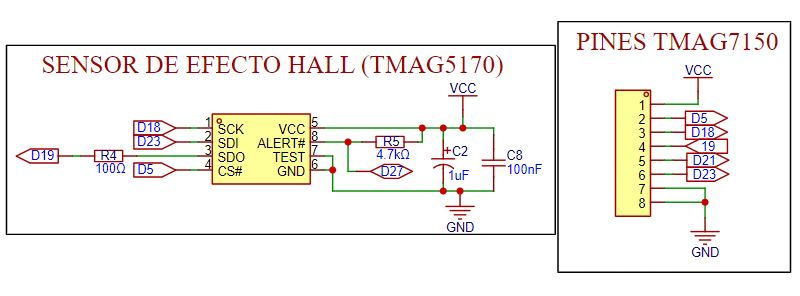
\includegraphics[width=1\textwidth]{CHPTRS/CH04_DIS_ELECTRONICO/Fig_Esquematicos/DIS_ELEC_05_CircuitoDeSensorTMAG7150.jpg}
           \caption{Diagrama esquemático con las conexiones del sensor de efecto \textit{hall}}
           \label{fig:switching}
        \end{figure}
        
        \medskip
        Configuración por registros (resumen). La programación detallada se desarrollará en el Capítulo de Pruebas de Prototipo; de forma resumida se configurarán:
        \begin{itemize}
          \item SENSOR\_CONFIG: habilitar X e Y, seleccionar el \textit{full-scale} por eje (por ejemplo, \(\pm 25/\pm 50/\pm 100\,\text{mT}\) en A1) y activar el cálculo de ángulo en \(XY\).
          \item DEVICE\_CONFIG y/o SYSTEM\_CONFIG: elegir el modo de conversión (continuo o por disparo), el promediado/\textit{oversampling} y, si aplica, el filtro digital para mejorar la relación señal–ruido.
          \item ALERT\_CONFIG: configurar ALERT como \textit{data-ready} para sincronizar la lectura desde la ESP32.
          \item Lectura periódica de ANGLE\_RESULT (o de BX/BY para cálculo con \(\operatorname{atan2}\)) y calibración de offset de cero.
        \end{itemize}

    \subsection{Diseño de circuitos de comunicación}
        El circuito implementa un puente USB–UART con el CH340 y un conector USB-C configurado como dispositivo mediante resistencias de 5.1 kohm en CC1/CC2; las líneas D+ y D$-$ se enrutan al CH340 con desacoplo local. El CH340 convierte los datos del PC a UART y enlaza TXD con RX0 y RXD con TX0 de la ESP32. Para el autoprogramado, las salidas DTR y RTS del CH340, a través de las redes R12/R15 y los transistores Q1/Q2 (con R11/R18 como limitadoras), fuerzan la secuencia de arranque: EN baja/alta mientras IO0 se mantiene bajo, entrando en modo bootloader; luego ambas retornan a alto por las pull-up R10 y R17 y el micro arranca en modo normal. Se incluyen pulsadores BOOT (IO0–GND) y RST (EN–GND) para control manual. Todas las masas comparten GND, y VBUS del conector alimenta la etapa mediante el regulador de la placa.
        \begin{figure}[H]
           \centering
           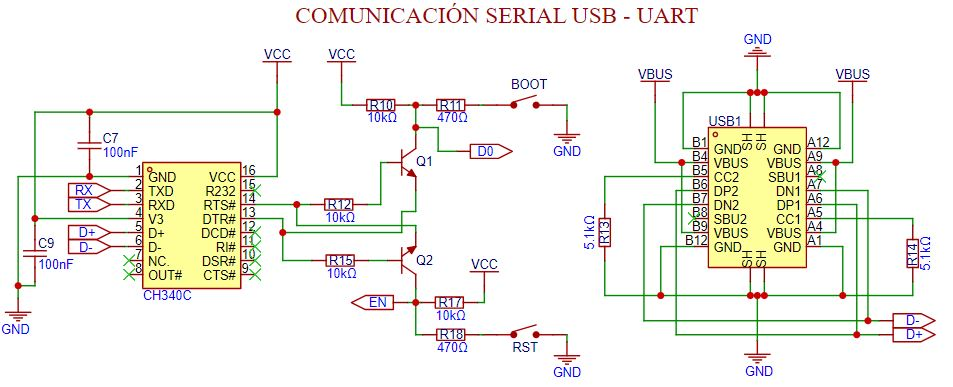
\includegraphics[width=1\textwidth]{CHPTRS/CH04_DIS_ELECTRONICO/Fig_Esquematicos/DIS_ELEC_02_CircuitoDeComunicacionPC.jpg}
           \caption{Diagrama esquemático del circuito de comunicación USB-UART}
           \label{fig:switching}
        \end{figure}
Finalmente, en la Tabla \ref{tab:pines_pcb} se presenta la distribución de pines del microcontrolador, con el fin de visualizar qué pines se utilizarán y configurar cada uno según su función en el programa que se cargará en la ESP32.

\begin{table}[H]
    \centering
    \caption{Pines utilizados en la PCB}
    \begin{tabularx}{0.92\textwidth}{l l X}
    \toprule
    Pin & Configuración & Función \\
    \midrule
    GPIO2  & GPIO (salida)          & LED ROJO \\
    GPIO4  & GPIO (entrada/INT)     & Interrupción (kill switch) \\
    GPIO5  & SPI (CS)               & CS SENSOR \\
    GPIO12 & GPIO (salida)          & SEL0 \\
    GPIO14 & ADC (entrada)          & ADC (MEDIR VOLTAJE de batería) \\
    GPIO18 & SPI (SCK)              & SCK \\
    GPIO19 & SPI (MISO)             & MISO \\
    GPIO22 & SPI (CS)               & CS PUERTO ETHERNET \\
    GPIO23 & SPI (MOSI)             & MOSI \\
    GPIO25 & PWM (LEDC)             & PWM driver \\
    GPIO27 & GPIO (entrada)         & STATUS OUTPUT TRIGERED \\
    IO32   & GPIO (salida)          & INA \\
    IO33   & GPIO (salida)          & INB \\
    GPIO34 & ADC (entrada)          & ADC (MEDIR CORRIENTE) \\
    \midrule
    TX     & UART (TX0)             & SUBIDA DE PROGRAMA \\
    RX     & UART (RX0)             & SUBIDA DE PROGRAMA \\
    D0     & BOOT           & SUBIDA DE PROGRAMA \\
    EN     & EN      & SUBIDA DE PROGRAMA \\
    \bottomrule
    \end{tabularx}
    \label{tab:pines_pcb}
\end{table}

% \section{Diseño de protocolo de comunicación con la interfaz con módulo Ethernet}

%     \begin{figure}[H]
%        \centering
%        \includegraphics[width=0.4\textwidth]{ethe}
%        \caption{\ac{PCB} de una fuente \textit{switching}}
%        \label{fig:switching}
%     \end{figure}
\section{Diagramas electrónicos}
    En esta sección se presenta el diagrama de conexiones entre la \ac{PCB} de control y la \ac{PCB} del sensor de efecto \textit{hall}. La Figura \ref{fig:pcb_control_full} muestra el esquema de la \ac{PCB} de control, mientras que la Figura \ref{fig:pcb_sensor_full} corresponde a la placa de adaptación del TMAG5170. En la sección siguiente se detallan los criterios de ruteo y el diseño final para su ensamble en el chasis.
    
    % Página 1 (figura rotada con leyenda rotada)
    \begin{sidewaysfigure}
      \centering
      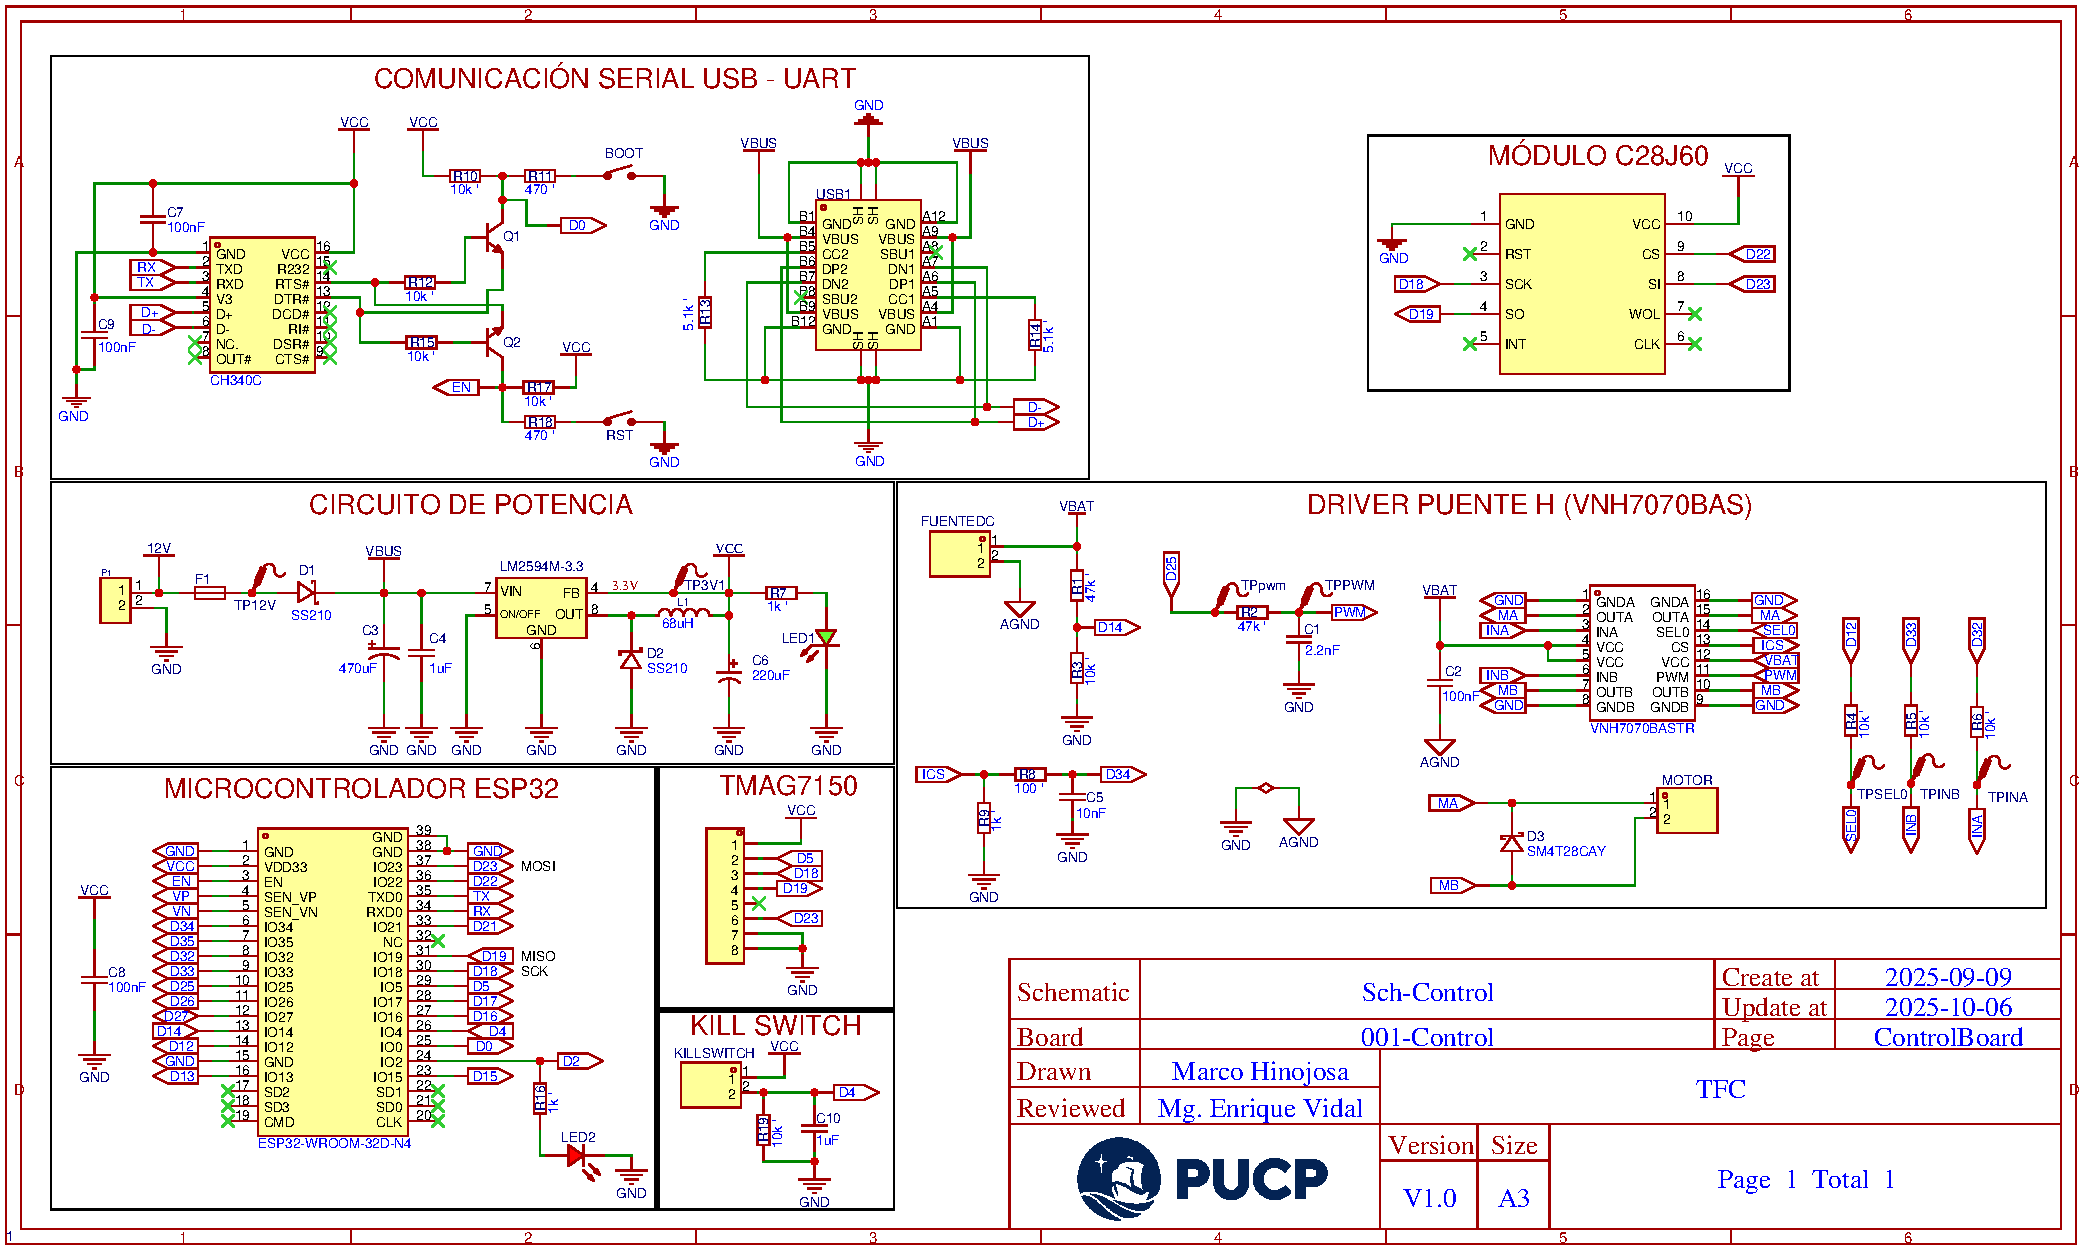
\includegraphics[width=\textheight]{CHPTRS/CH04_DIS_ELECTRONICO/Fig_Esquematicos/DIS_ELEC_06_DiagramaEsquematico.pdf}
      \caption{Diagrama esquemático general para la \ac{PCB} de control}
      \label{fig:pcb_control_full}
    \end{sidewaysfigure}
    
    % Página 2 (figura rotada con leyenda rotada)
    \begin{sidewaysfigure}
      \centering
      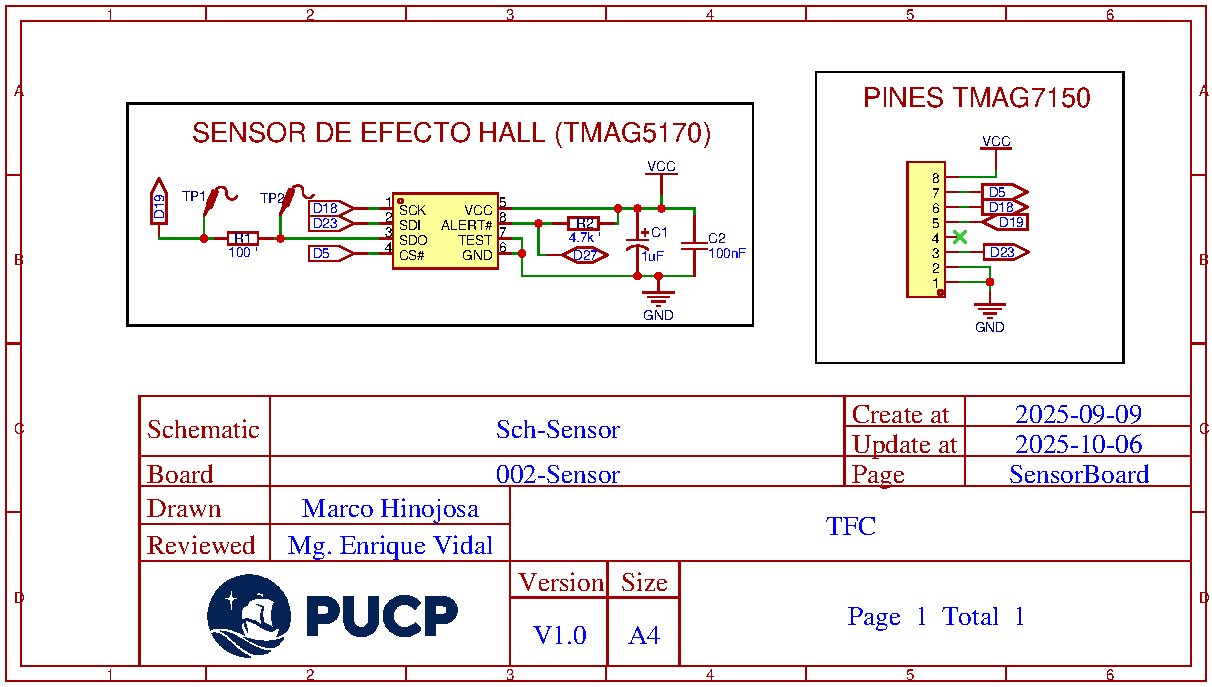
\includegraphics[width=\textheight]{CHPTRS/CH04_DIS_ELECTRONICO/Fig_Esquematicos/DIS_ELEC_07_DiagramaEsquematicoSensor.pdf}
      \caption{Diagrama esquemático con las conexiones del sensor de efecto \textit{hall}}
      \label{fig:pcb_sensor_full}
    \end{sidewaysfigure}

\section{Diseño de las \ac{PCB}s}
    Con base en lo anterior, se procede al ruteo de la \ac{PCB}. Se aplican las recomendaciones del fabricante y los criterios de integridad térmica y eléctrica. En particular, para el VNH7070BAS se siguen las pautas de disipación y almohadillas térmicas mostradas en la Figura \ref{fig:layerVNH7070BAS}.

    \begin{figure}[H]
       \centering
       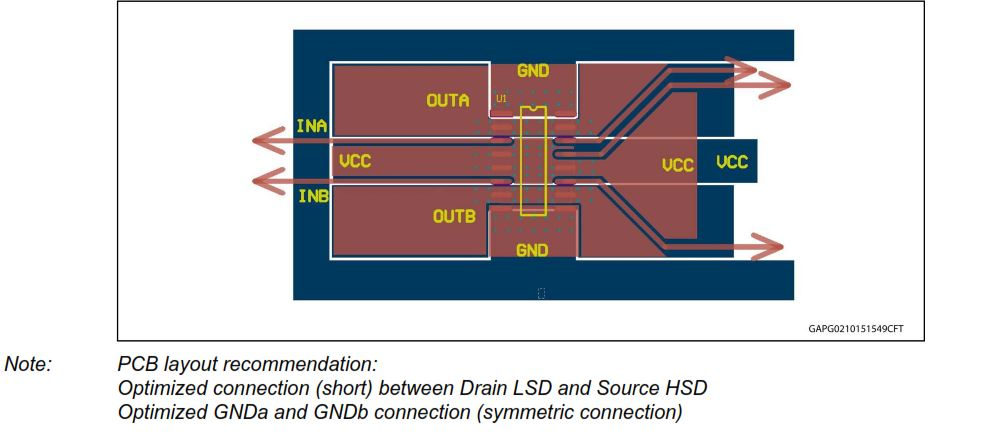
\includegraphics[width=0.8\textwidth]{CHPTRS/CH04_DIS_ELECTRONICO/Fig_DiseñoPCB/LayerVNH7070BAS.JPG}
       \caption{Recomendación del fabricante respecto a las \textit{layers} superficies de disipación y trazas del driver VNH7070BAS}
       \label{fig:layerVNH7070BAS}
    \end{figure}
    
    Asimismo, se define la ubicación de conectores y la distribución de componentes en el chasis, priorizando recorridos de cable cortos, accesibilidad a alimentación, comunicación y mandos, y evitando cruces. La Figura \ref{fig:Distribución de componentes} presenta un esquema con una vista superior con las salidas hacia la \ac{PCB} y la ubicación de los elementos del chasis.
    
    \begin{figure}[H]
       \centering
       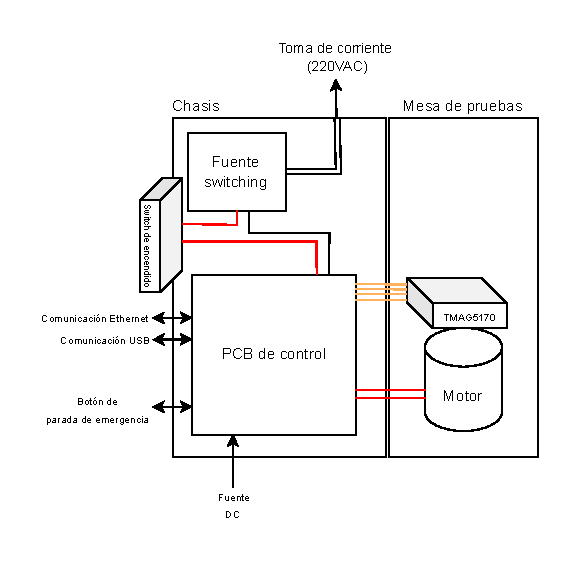
\includegraphics[width=0.8\textwidth]{CHPTRS/CH04_DIS_ELECTRONICO/Fig_Esquematicos/DistribuciónDeComponentes.pdf}
       \caption{Distribución de componentes y conectores (vista superior)}
       \label{fig:Distribución de componentes}
    \end{figure}
    
    El ancho de pista se dimensiona con el modelo IPC-2221. Para una corriente \(I\) y un aumento de temperatura objetivo \(\Delta T\):
    \begin{align*}
      A~[\text{mil}^2] &= \left(\frac{I~[\text{A}]}{k\,(\Delta T~[^\circ\text{C}])^{b}}\right)^{\tfrac{1}{c}},\\
      W~[\text{mil}] &= \frac{A~[\text{mil}^2]}{t_\text{cu}~[\text{mil}]},
    \end{align*}
    Donde, para las capas externas, k = 0.048, b = 0.44, c = 0.725 y el espesor de cobre es 1.378 mil (1 oz por pie cuadrado).\footnote{1 mil equivale a 0,0254 mm; 1 oz por pie cuadrado equivale aproximadamente a 1,37 a 1,378 mil, es decir, cerca de 35 micrómetros.} Para las capas internas se usa k = 0.024 y se mantienen los mismos valores de b y c \cite{DigiKey_TraceWidth}.

    Se considerará un diseño de \ac{PCB} de dos capas con cobre de 1 oz. Asimismo, se asumirá una temperatura ambiente de 25 °C y una elevación térmica de 25 °C.

    \begin{table}[H]\centering
    \caption{Ancho mínimo por corriente (IPC-2221, 1 oz, capa externa, \(\Delta T=25~^\circ\text{C}\)).}
    \begin{tabular}{rcc}
    \toprule
    Corriente & Ancho mínimo [mil] & Ancho mínimo [mm]\\
    \midrule
    0.01 A  & 0.012  & 0.0003 \\
    0.05 A  & 0.109  & 0.0028 \\
    0.10 A  & 0.283  & 0.0072 \\
    0.50 A  & 2.607  & 0.0662 \\
    1.00 A  & 6.781  & 0.1723 \\
    1.50 A  & 11.863 & 0.3013 \\
    2.00 A  & 17.642 & 0.4481 \\
    3.00 A  & 30.862 & 0.7839 \\
    5.00 A  & 62.434 & 1.5858 \\
    \bottomrule
    \end{tabular}
    \end{table}
    
    Notas: (1) Para corrientes pequeñas, el límite lo impone la capacidad de fabricación (por ejemplo, 0.30 mm), no la fórmula. (2) Si se desea menor \(\Delta T\), el ancho requerido aumenta; con 2 oz, el ancho se reduce aproximadamente a la mitad para la misma \(I\).
        
    \subsection*{Criterios prácticos y refuerzos}
        \begin{itemize}
          \item En zonas de potencia de motor, usar polígonos/planos; dejar la pista sin máscara para estañar y aumentar sección cuando sea posible.
          \item Para pasos entre capas en líneas de potencia, colocar múltiples vías en paralelo (via stitching).
          \item Mantener tramos cortos y anchos desde el conector de 12 V hasta el condensador de reserva del driver y desde OUTA/OUTB al bornero del motor; cerrar retornos en un punto estrella de potencia.
        \end{itemize}
    
    \subsection*{Anchos adoptados para esta PCB (1 oz)}
        % Requiere: \usepackage{tabularx,booktabs,array}
    \begin{table}[H]
    \centering
    \caption{Anchos seleccionados por red (consideran mínimo de fábrica y margen térmico).}
    \setlength{\tabcolsep}{5pt}
    \renewcommand{\arraystretch}{1.1}
    \footnotesize
    \begin{tabularx}{0.95\linewidth}{@{}>{\raggedright\arraybackslash}X
                                        >{\raggedright\arraybackslash}l
                                        >{\raggedright\arraybackslash}X@{}}
    \toprule
    \textbf{Red / función} & \textbf{Ancho adoptado} & \textbf{Justificación} \\
    \midrule
    Señales digitales (GPIO, SPI, PWM, ALERT) & 12 mil (0.30 mm) & Mínimo de fábrica; \(I \ll 10\) mA \\
    3.3 V — tramo principal (hasta 1.5 A)     & 24 mil (0.61 mm) & Cálculo 11.86 mil; se duplica por margen \\
    3.3 V — ramales a cargas (ESP32, ENC28J60, TMAG) & 12 mil (0.30 mm) & Corrientes \(\leq\) 0.5 A por ramal; cálculo 2.61 mil \\
    GND (control)                              & Plano            & Menor impedancia y retorno controlado \\
    12 V — entrada (conector → driver)         & 80 mil (2.03 mm) & Margen sobre cálculo 5 A = 62.4 mil; tramo corto y ancho \\
    OUTA/OUTB → bornero motor                  & 100 mil (2.54 mm) + polígono/estañado & Robustez, baja caída; admite picos \\
    Sense y señales analógicas                 & 12 mil (0.30 mm) & Separación de lazos de potencia \\
    \bottomrule
    \end{tabularx}
    \label{tab:anchos_pcb}
    \end{table}

        
        En caso de limitaciones de espacio, priorizar polígonos para potencia y mantener la máscara abierta en los “bus bars” para añadir estaño en el ensamblaje y aumentar la sección.

    
\section{\textit{Layers} de la PCB}
    Este capítulo de diseño electrónico concluye con la presentación de los layers y las vistas \ac{CAD} del diseño de la \ac{PCB} de control y de la \ac{PCB} de sensado de velocidad. Sus dimensiones se tomarán como referencia en el Capítulo \ref{ch:CH04-Diseno-Mecanico}, dedicado al ensamblaje en el chasis. En la Figura \ref{fig:Layers} se muestran las imágenes finales de las tarjetas.
    \begin{figure}[H]
        \begin{tabularx}{\linewidth}{*{2}{>{\centering\arraybackslash}X}}
            % FILA-1, COL-1.
            \begin{subfigure}[t]{0.45\textwidth}
                \centering
                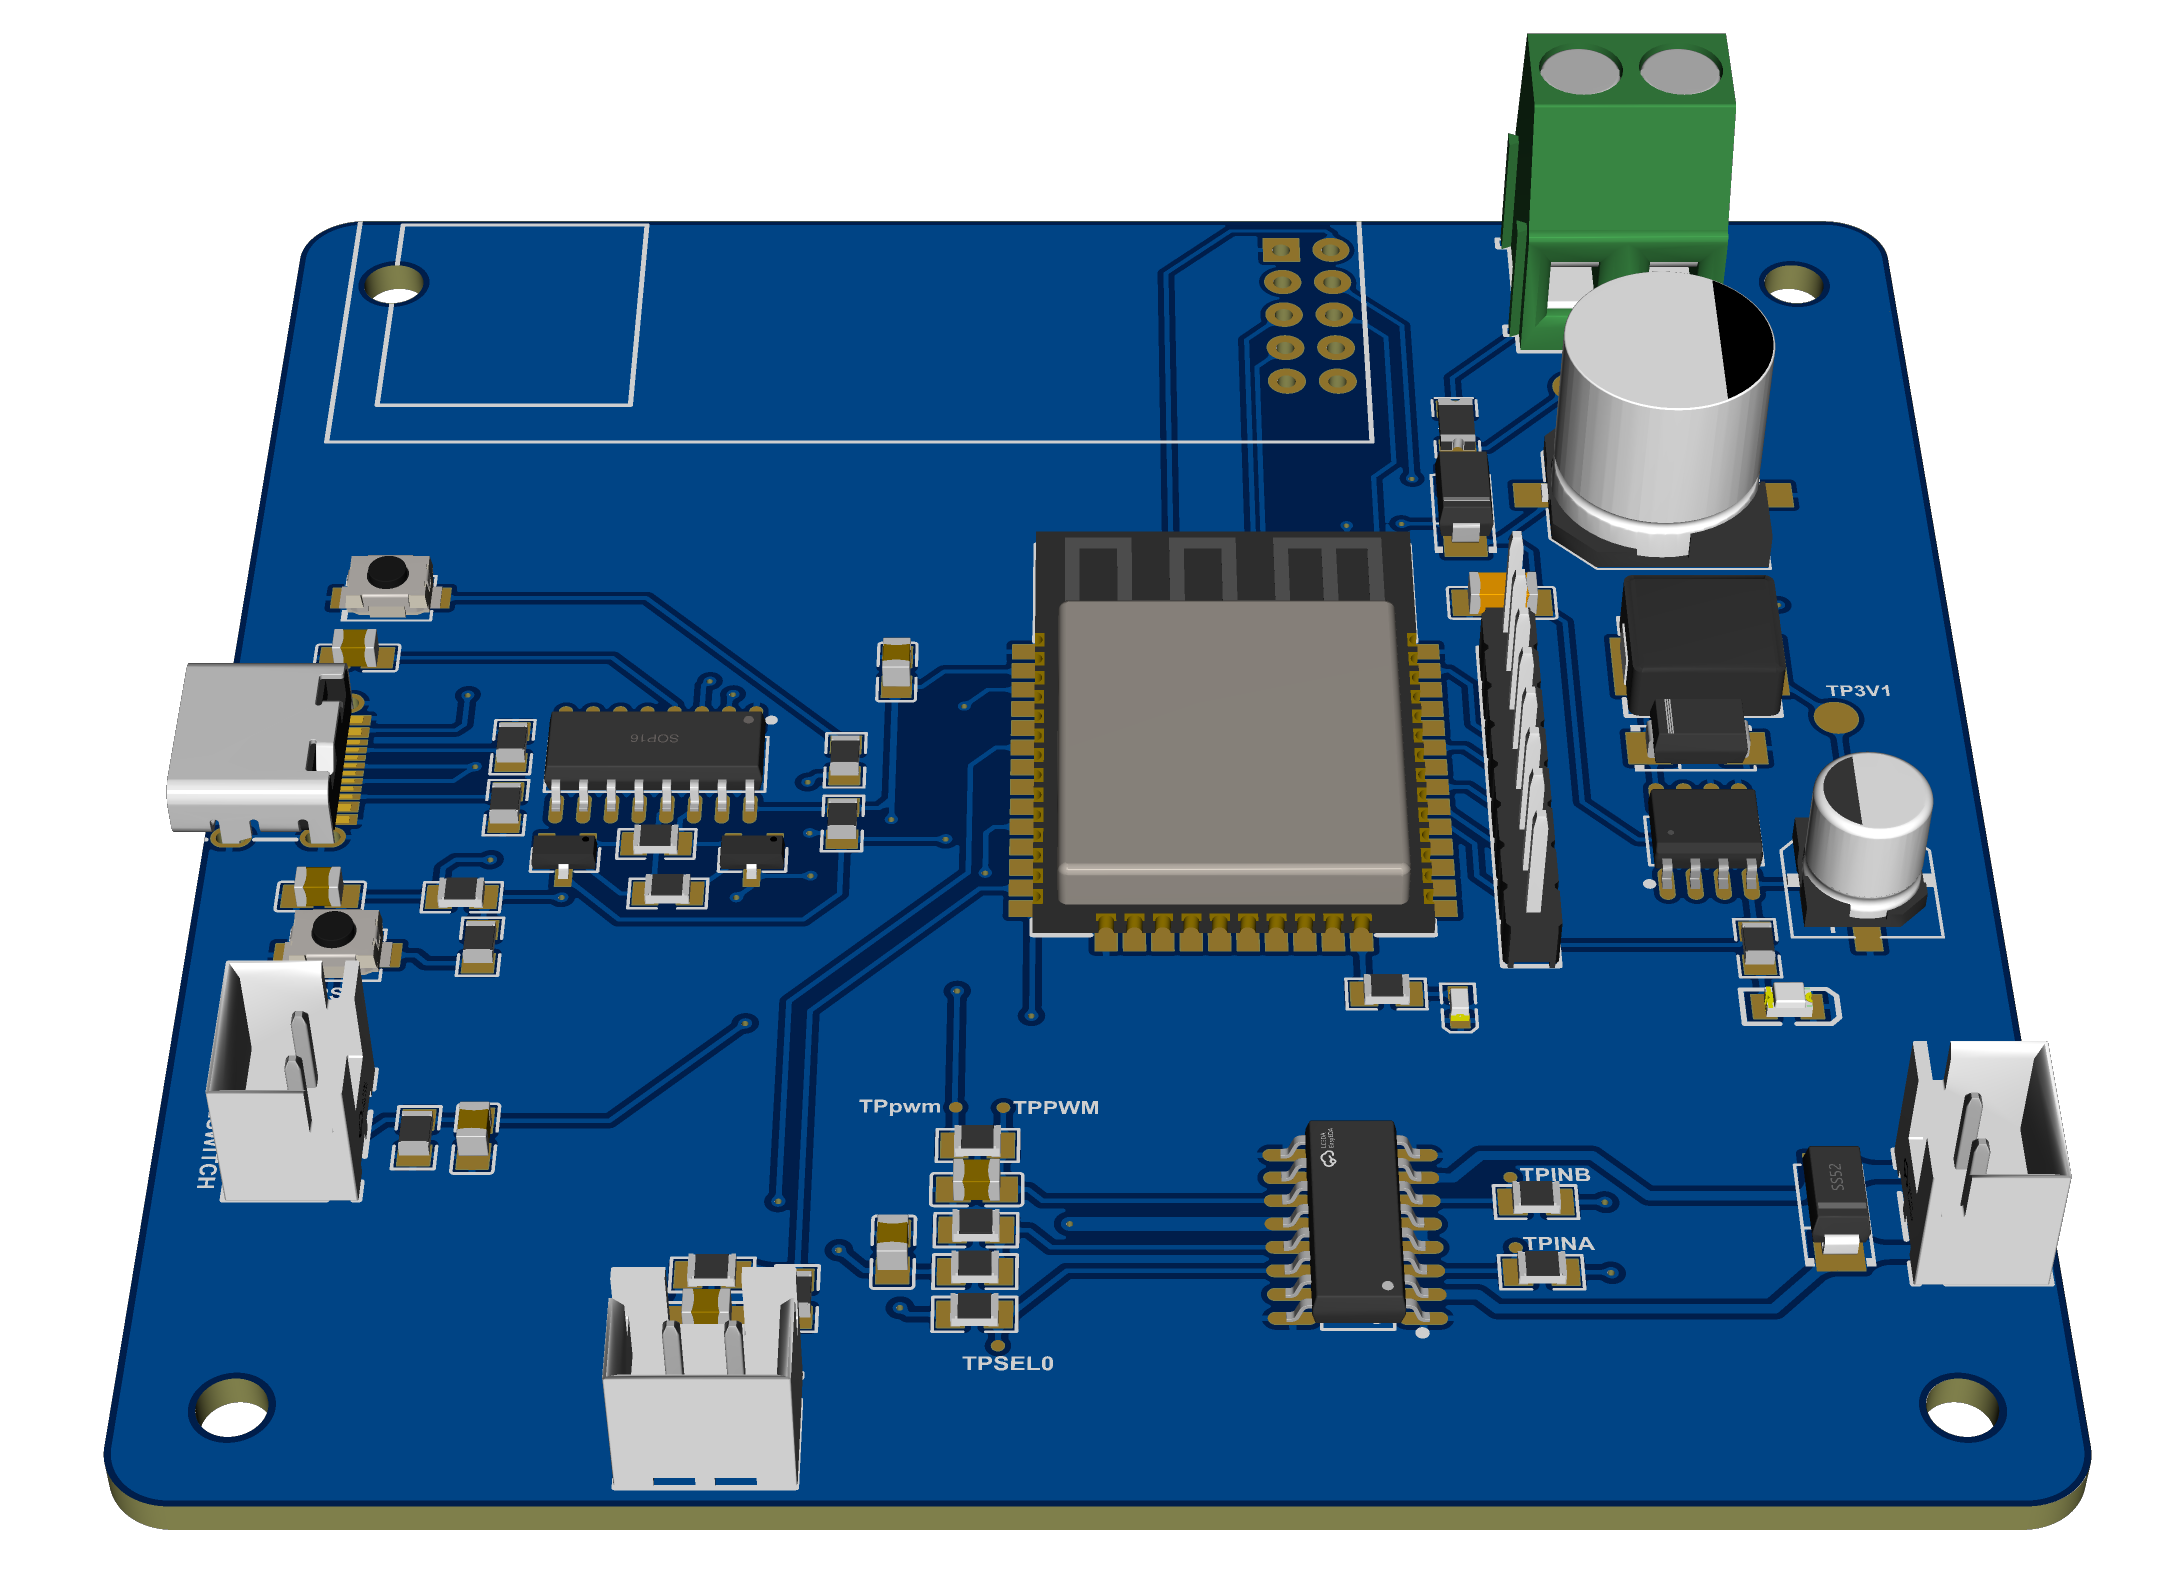
\includegraphics[width=.9\linewidth]{CHPTRS/CH04_DIS_ELECTRONICO/Fig_Esquematicos/PCB_control.png}
                %\label{fig:imagen_pcb_control} %LABEL ESTA DESPUES
            \end{subfigure}
            & %Nueva Columna, es decir: % FILA-1, COL-2
            \begin{subfigure}[t]{0.45\textwidth}
                \centering
                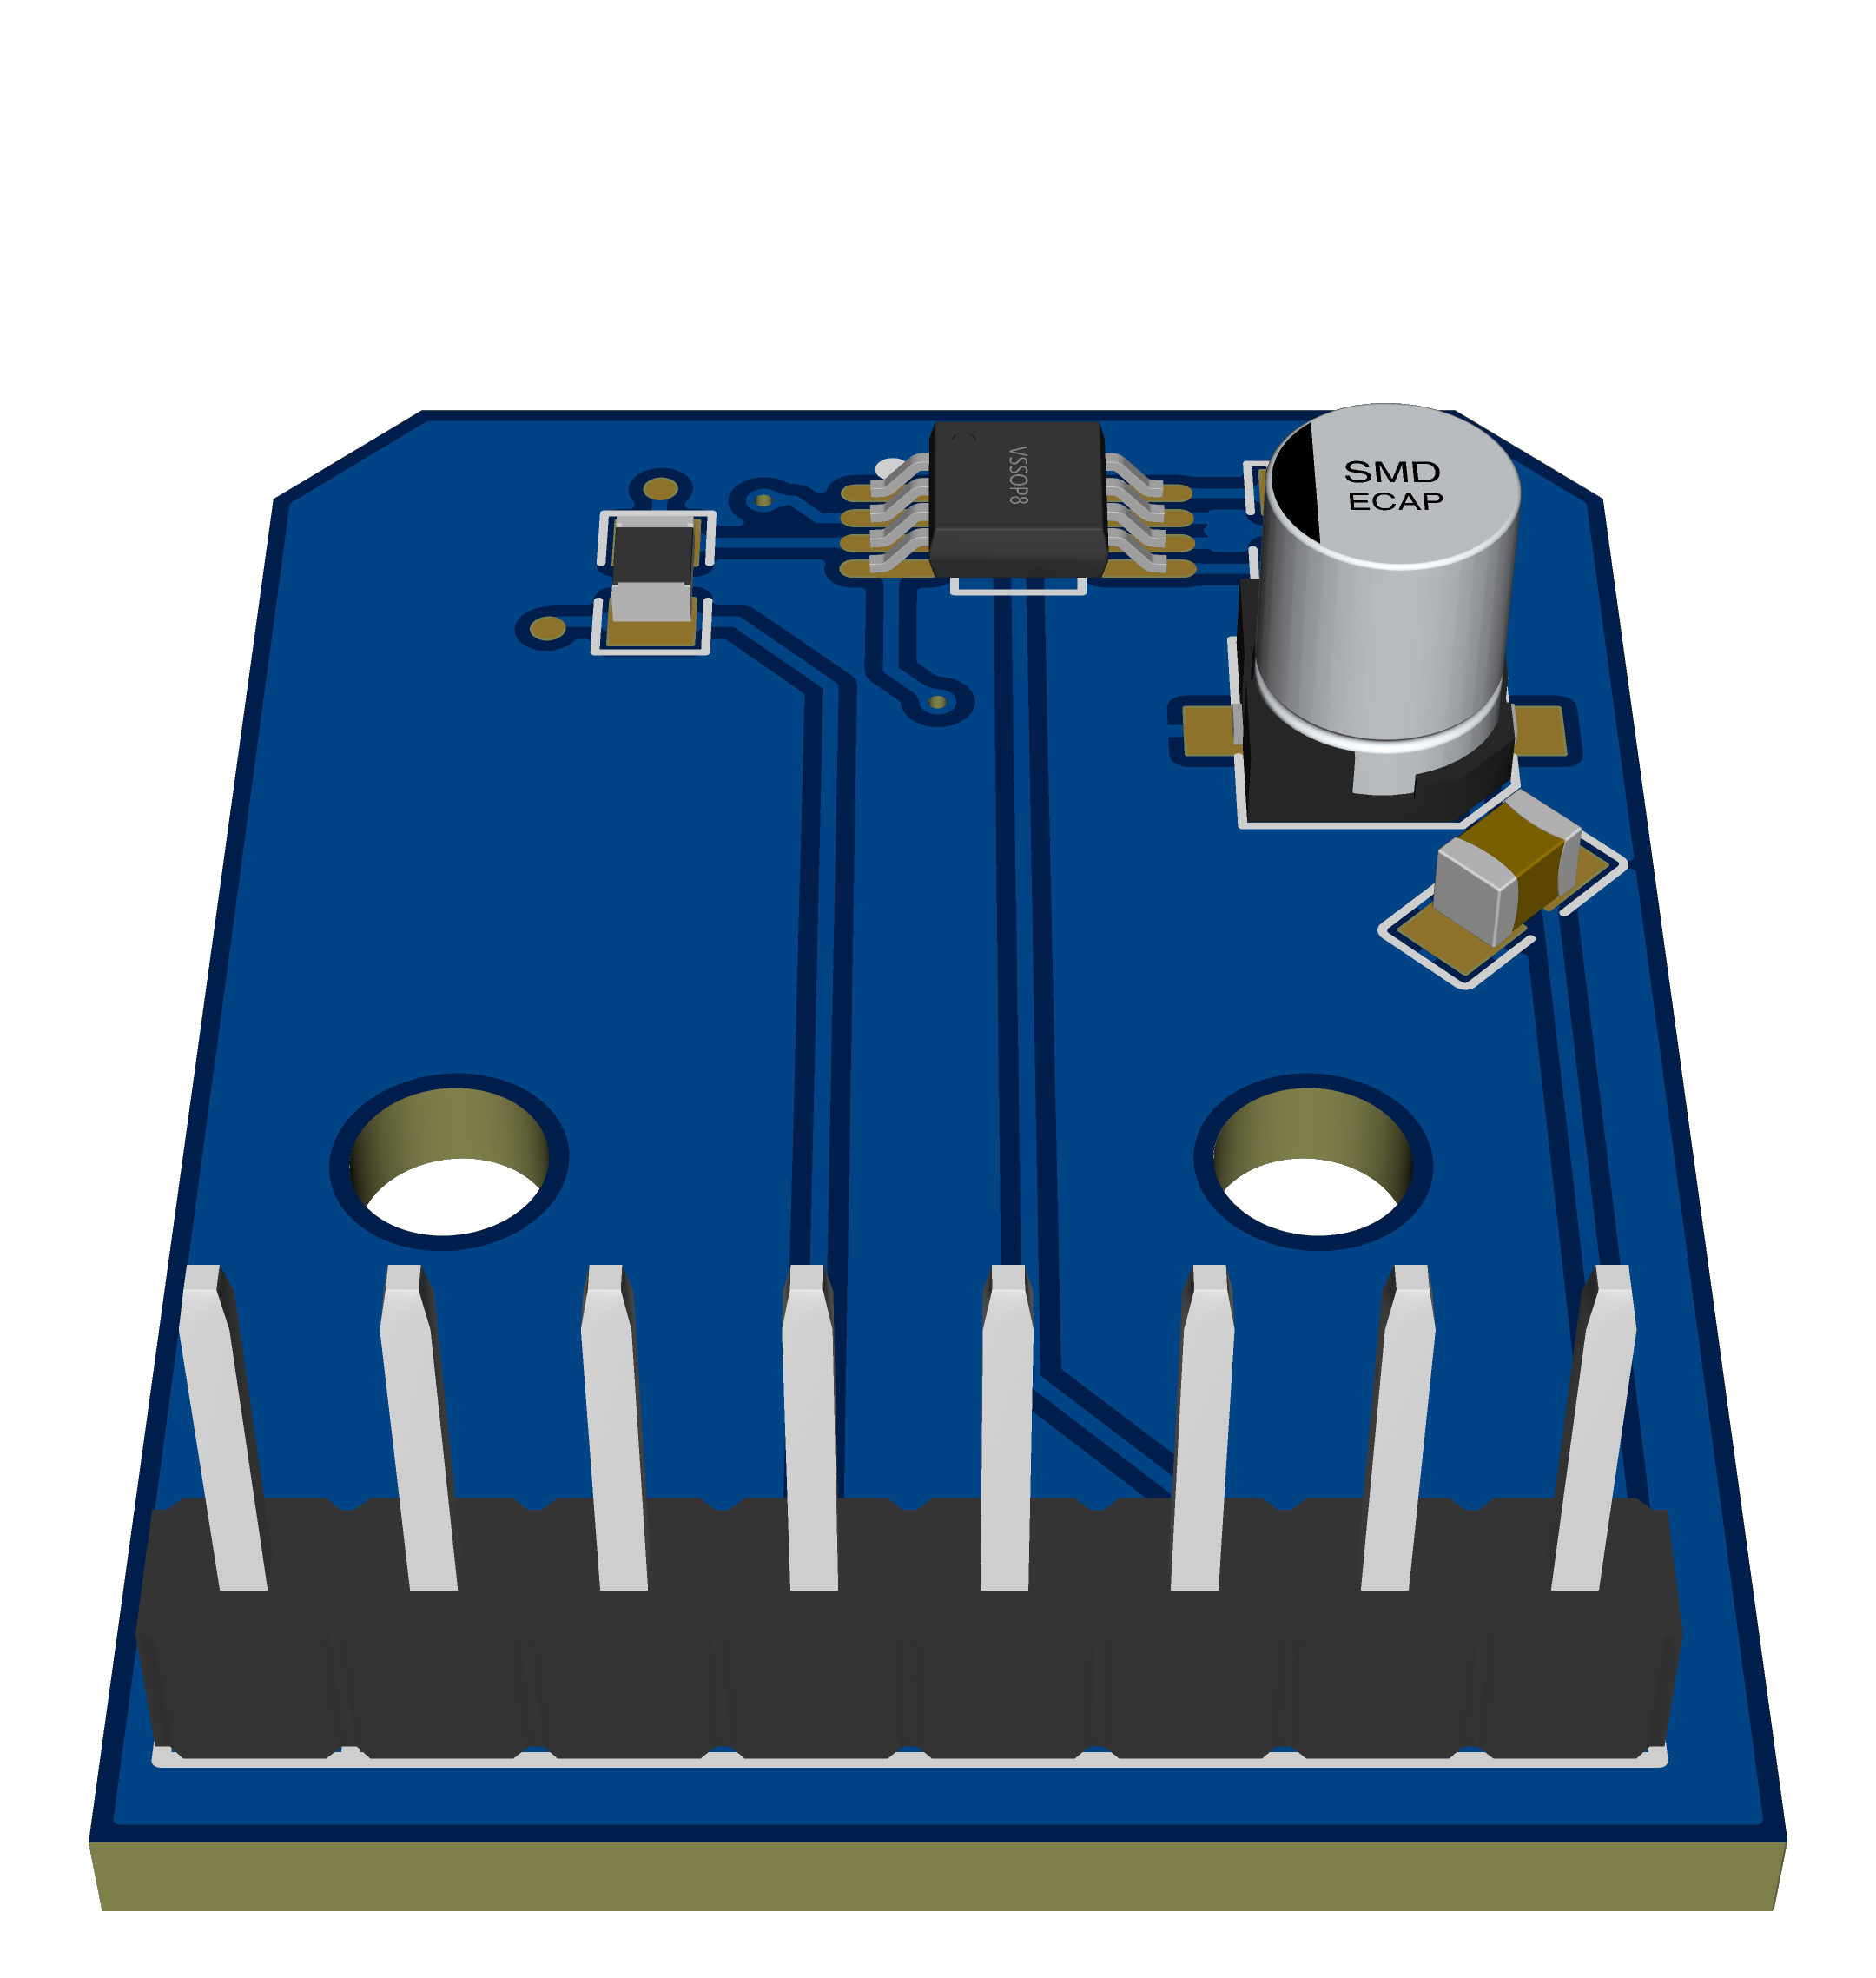
\includegraphics[width=.68\linewidth]{CHPTRS/CH04_DIS_ELECTRONICO/Fig_Esquematicos/PCB_sensor.png}
            \end{subfigure}
            \\ %Nueva Fila, es decir: % FILA-2, COL-1
            \begin{subfigure}[t]{0.8\linewidth}
                \caption{Imagen referencial de cómo quedará la \ac{PCB} de control}
                \label{fig:romeo}
            \end{subfigure} 
            & %Nueva Columna, es decir: % FILA-2, COL-2
            \begin{subfigure}[t]{0.8\linewidth}
                \caption{Imagen referencial de cómo quedará la \ac{PCB} para el sensor de efecto \textit{hall}}
                \label{fig:imagen_pcb_tmag5170}
            \end{subfigure}
        \end{tabularx}
        \caption{Vista general de las\ac{PCB}s de control y la de \textit{encoder}}
        \label{fig:Layers}
    \end{figure}